
\pagelayout{wide} % No margins
% \myepigraphhead[500]{Of all humanity's instruments, the most wondrous, no
% doubt, is the book. The other instruments are extensions of his body. The
% microscope, the telescope, are extensions of his sight; the telephone is the
% extension of his voice; then we have the plow and the sword, extensions of the
% arm. But the book is something else altogether: the book is an extension of
% memory and imagination.\\//\\De los diversos instrumentos del hombre, el más
% asombroso es, sin duda, el libro. Los demás son extensiones de su cuerpo. El
% microscopio, el telescopio, son extensiones de su vista; el teléfono es
% extensión de la voz; luego tenemos el arado y la espada, extensiones de su
% brazo. Pero el libro es otra cosa: el libro es una extensión de la memoria y
% de la imaginación.}{Jorge Luis Borges}
\myepigraphhead[500]{I, who was never even sure what time it was, nodded with the conviction of the ignorant.\\//\\Yo, que nunca estaba seguro ni de la hora que era, asentí con la convicción del ignorante.}{Carlos Ruiz Zafón, \textit{The Shadow of the Wind // La Sombra del Viento}}
\part{Optimal water and electricity management in a combined cooling system}

% \section*{TL;DR}
% \addcontentsline{toc}{section}{TL;DR}

\glsresetall % Reset glossary entries

\tldrbox{ 
%     To enhance the applicability and sustainability of solar thermal
% technologies, this work investigates a novel cooling system for the power block
% of a \gls{cspLabel} plant, combining dry and wet cooling components. A model of
% the \gls{ccsLabel} was developed alongside a two-stage optimization strategy.
% The methodology was validated using an experimental pilot plant, achieving R$^2$
% values above 0.9 for the main output variables and successfully adapting the
% plant's operation to changing conditions.

% A case study is presented for a commercial 50~MW$_\text{e}$ CSP plant with 8 hours
% of storage, Andasol-II, using annual simulations under a water-scarcity
% scenario where the current wet-only cooling system is replaced with the proposed
% \gls{ccsLabel}. Results indicate a potential 80~\% reduction in cooling costs
% and a 48~\% reduction in mean annual water use, but more importantly, a 38~\%
% reduction during the driest and hottest months, demonstrating the significant
% potential of the system when operated optimally. \\

This part of the thesis addresses the challenge of reducing water consumption in
\gls{cspLabel} plants through a hybrid cooling concept combining dry and wet
technologies. The broader context of concentrated solar thermal power and its
dependence on water resources is introduced, motivating more water-efficient
cooling solutions. An experimental \gls{ccLabel} pilot plant at \gls{psaLabel}
is then presented, comprising a \gls{wctLabel} and a \gls{dcLabel} integrated
with a surface condenser in a flexible-hydraulic circuit.\\

A steady-state modelling framework is developed for the main components of the
combined cooler. Two complementary strategies are considered: physics-based
first-principles models with broad applicability, and several data-driven
approaches (artificial neural networks, Random Forest, Gradient Boosting, and
Gaussian Process Regression). To combine the generality of physical models with
the speed of data-driven surrogates, Gaussian Process models are trained on
synthetic data generated by first-principles simulations. This yields fast,
scalable surrogate models with high predictive accuracy, achieving mean absolute
errors below 0.97~$^\circ$C for key temperatures and 19.4~L/h for water
consumption when validated against 24 experimental tests over a wide operating
range.\\

Building on this framework, a two-stage multi-objective optimization strategy is
proposed to minimize daily cooling cost ---electricity and water--- under
limited water availability while ensuring the required cooling duty. At each
time step, a multi-objective problem generates a Pareto front between cost and
water use; a second-stage optimization selects an optimal path across the
horizon. Pilot-plant validation shows very good agreement between optimized and
measured operation. The results highlight the strong sensitivity of dry cooling
to ambient temperature, the wet cooler's compensating role when dry cooling
reaches its limits, and the systematic prioritization of water savings,
including periods of dry-only or series operation. Tests also show that the
optimized strategies remain valid for extended quasi-steady periods, and that
upper-layer predictions can support low-level control (\eg\ feed-forward
actions), improving robustness when re-optimization is delayed.\\

The methodology is then applied to a case study of a commercial 50~MW$_\text{e}$
\gls{cspLabel} plant with 8~h of storage (Andasol-II, southern Spain). Three
cooling configurations are compared under a water-scarcity scenario using annual
simulations: the existing wet-only \gls{wctLabel}, and two \gls{ccLabel}
variants with dry-cooler capacities of 75~\% and 100~\% of the nominal wet load.
For each configuration, operation is optimized using the proposed framework. The
combined-cooler options reduce specific cooling costs by up to 80~\% and annual
water consumption by about 48~\%, with 38~\% savings during the driest and
hottest months. These gains stem mainly from reduced reliance on expensive
alternative water sources. The \gls{ccLabel} configurations also show more
stable and predictable annual costs than the water-sensitive wet-only
reference.\\

The analysis underscores the importance of evaluating cooling concepts over
representative annual conditions rather than relying on aggregated averages, and
confirms that water availability can become the dominant constraint and cost
driver, especially where alternative sources are costly. Although no strategy
can fully resolve the mismatch between peak cooling demand and water scarcity in
hot-dry seasons, the results demonstrate substantial potential for improved
water management through optimized hybrid-cooling operation. The proposed
framework is generic and adaptable to other plant designs, locations, and
resource scenarios, supporting informed decisions for more sustainable
\gls{cspLabel} plants.\\

\centering
\begin{minipage}{.98\linewidth}
    \centering
    \includegraphics[width=\linewidth]{cc-visual-abstract-with-results.png}\\
    \small \textit{Visual abstract}
\end{minipage}
}
% \section*{Derived scientific contributions}
% \addcontentsline{toc}{section}{Derived scientific contributions}


\section*{Part structure}

This part is structured as follows: first in \nrefch{cc:intro} a context of
concentrated solar thermal technologies is provided and their relationship with
the water resource, specifically for the case of \gls{cspLabel}. Then, the
experimental \gls{ccsLabel} pilot at \gls{psaLabel} is presented in
\refch{cc:facility}. The methodology for modelling and optimizing the operation
of the system are described in \refch{cc:modelling} and \refch{cc:optimization},
respectively. The validation with experimental data is shown in
\refch{cc:validation}. Finally, \refch{cc:simulation}, describes and analyzes
the results of the annual simulations performed for a commercial \gls{cspLabel}
plant, Andasol-II, using the proposed cooling system.

\pagelayout{margin} % Restore margins
%===================================
%===================================
%===================================
\setchapterpreamble[u]{\margintoc}
\chapter{Solar thermal energy and water}
\labch{cc:intro}

\tldrbox{
In the pursuit of eliminating reliance on fossil fuels sources for energy
generation and replacing them by renewable sources, \fullgls{cspLabel}
has proven to be a reliable contributor. In particular, in providing much
needed energy storage, dispatchability and ensuring grid stability. \\

However, water availability emerges not only as a technical constraint
but also as a planning and policy issue. \gls{cspLabel} deployment in water-stressed
regions is strongly dependent on innovative cooling solutions, policy
incentives, and careful water resource management to ensure sustainable
operation without compromising water security for local communities.\\

Ideally, negligible raw water would be needed to operate a \gls{cspLabel} plant
and it should be achieved with no increase in the \gls{lcoeLabel}. The most
water demanding component is the cooling of the power block, and currently this
water saving can be achieved with dry cooling and an increase of 7\% in the
\gls{lcoeLabel}. A compromise solution can be reached by using hybrid
cooling solutions together with water preservation strategies.

% , achieving an 83\%
% decrease in raw water consumption with respect to wet cooling with no reuse and
% a 5\% increase in the \gls{lcoeLabel}~\cite{rohani_optimization_2021}.\\

Further savings can be achieved by optimizing the operation of the hybrid
cooler and take full advantage of its flexibility towards optimal resource
management.
}


%===================================
%===================================
\section{Concentrated solar thermal}

% Introduction to solar thermal

\fullgls{cstLabel} technologies use heliostats or mirrors to reflect
and concentrate solar radiation onto a receiver. There, the radiation is
captured as heat, also known as thermal energy. They can be classified in
different ways\sidenote{With some parameters being correlated; for example,
higher operating temperatures generally mean higher concentration factors},
using temperature, two broad groups can be identified.

\begin{figure*}
    \centering
    \subfloat[\centering Parabolic trough pilot plant at \gls{psaLabel}]{{\includegraphics[width=0.48\linewidth]{parabolic-through-pt100-psa.jpg}}}%
    \hspace{0.01\linewidth}
    \subfloat[\centering Gemasolar 20MW$_\text{e}$-15h central tower \gls{cspLabel} plant in Sevilla,
    Spain.\\Source:
    \href{https://commons.wikimedia.org/wiki/File:Gemasolar_Thermosolar_Plant_2.jpg}{Wikipedia}]{{\includegraphics[width=0.48\linewidth]{solar-tower-gemasolar.png}}}%
    \caption[Two main \gls{cstLabel}
    technologies]{Two main \gls{cstLabel}
    technologies. In (a) collector rows positioned facing each other for
    cinematographic purposes}
    \labfig{cc:intro:cst-technologies}
\end{figure*}


The first group includes lower-temperature systems operating below
400~$^\circ$C. These are typically used for applications such as power
generation, district heating, cooling, and desalination. It is worth noting that
most industrial heat demand lies within this relatively low-temperature range of
100--400~$^\circ$C~\sidecite{schoeneberger_solar_2020}. This segment of
\gls{cstLabel} is also the most technically mature. Over the past decades,
considerable progress has been made in line-focus technologies such as parabolic
troughs (see \reffig{cc:intro:cst-technologies} (a)) and linear Fresnel
collectors\sidenote[][*-1]{Flat-plate collectors, though non-concentrating also
deserve mention here, as they remain the most widely deployed solar thermal
technology~\cite{ieashc_solar_2025}}. Although these systems have reached a high
level of development, their potential for significant further cost reduction is
relatively limited.

The second group comprises high-temperature systems operating above
600~$^\circ$C. These rely on point-focus technologies, most notably central
receiver systems similar to the one shown in
\reffig{cc:intro:cst-technologies}~(b). They can reliably
operate below 600~$^\circ$C but above ---and using a Brayton cycle--- are still
under development. They show promising potential for higher-value applications,
including solar-driven chemical processes (such as aviation fuel production) and
the provision of high-grade industrial heat in sectors like cement
manufacturing~\sidecite{thonig_concentrating_2023}. Central receiver technology,
however, remains at an earlier stage of commercial maturity. Fewer plants have
been built, and many existing installations employ a mix of technical
approaches~\sidecite{mehos_concentrating_2020}.


%================================
\subsection{\gls{cspLabel}: Concentrated Solar Power}
\labsec{cc:intro:csp:working-principle}

In a concentrated solar power plant, power is generated with a power-cycles such
as Rankine or Brayton. The principle of operation is very similar to
conventional thermal power plant, however, the working fluid is heated up not by
combusting/burning a fossil fuel, but as mentioned, by concentrating solar
energy as shown in \reffig{cc:intro:csp-plant-diagram}. 

\begin{figure}
    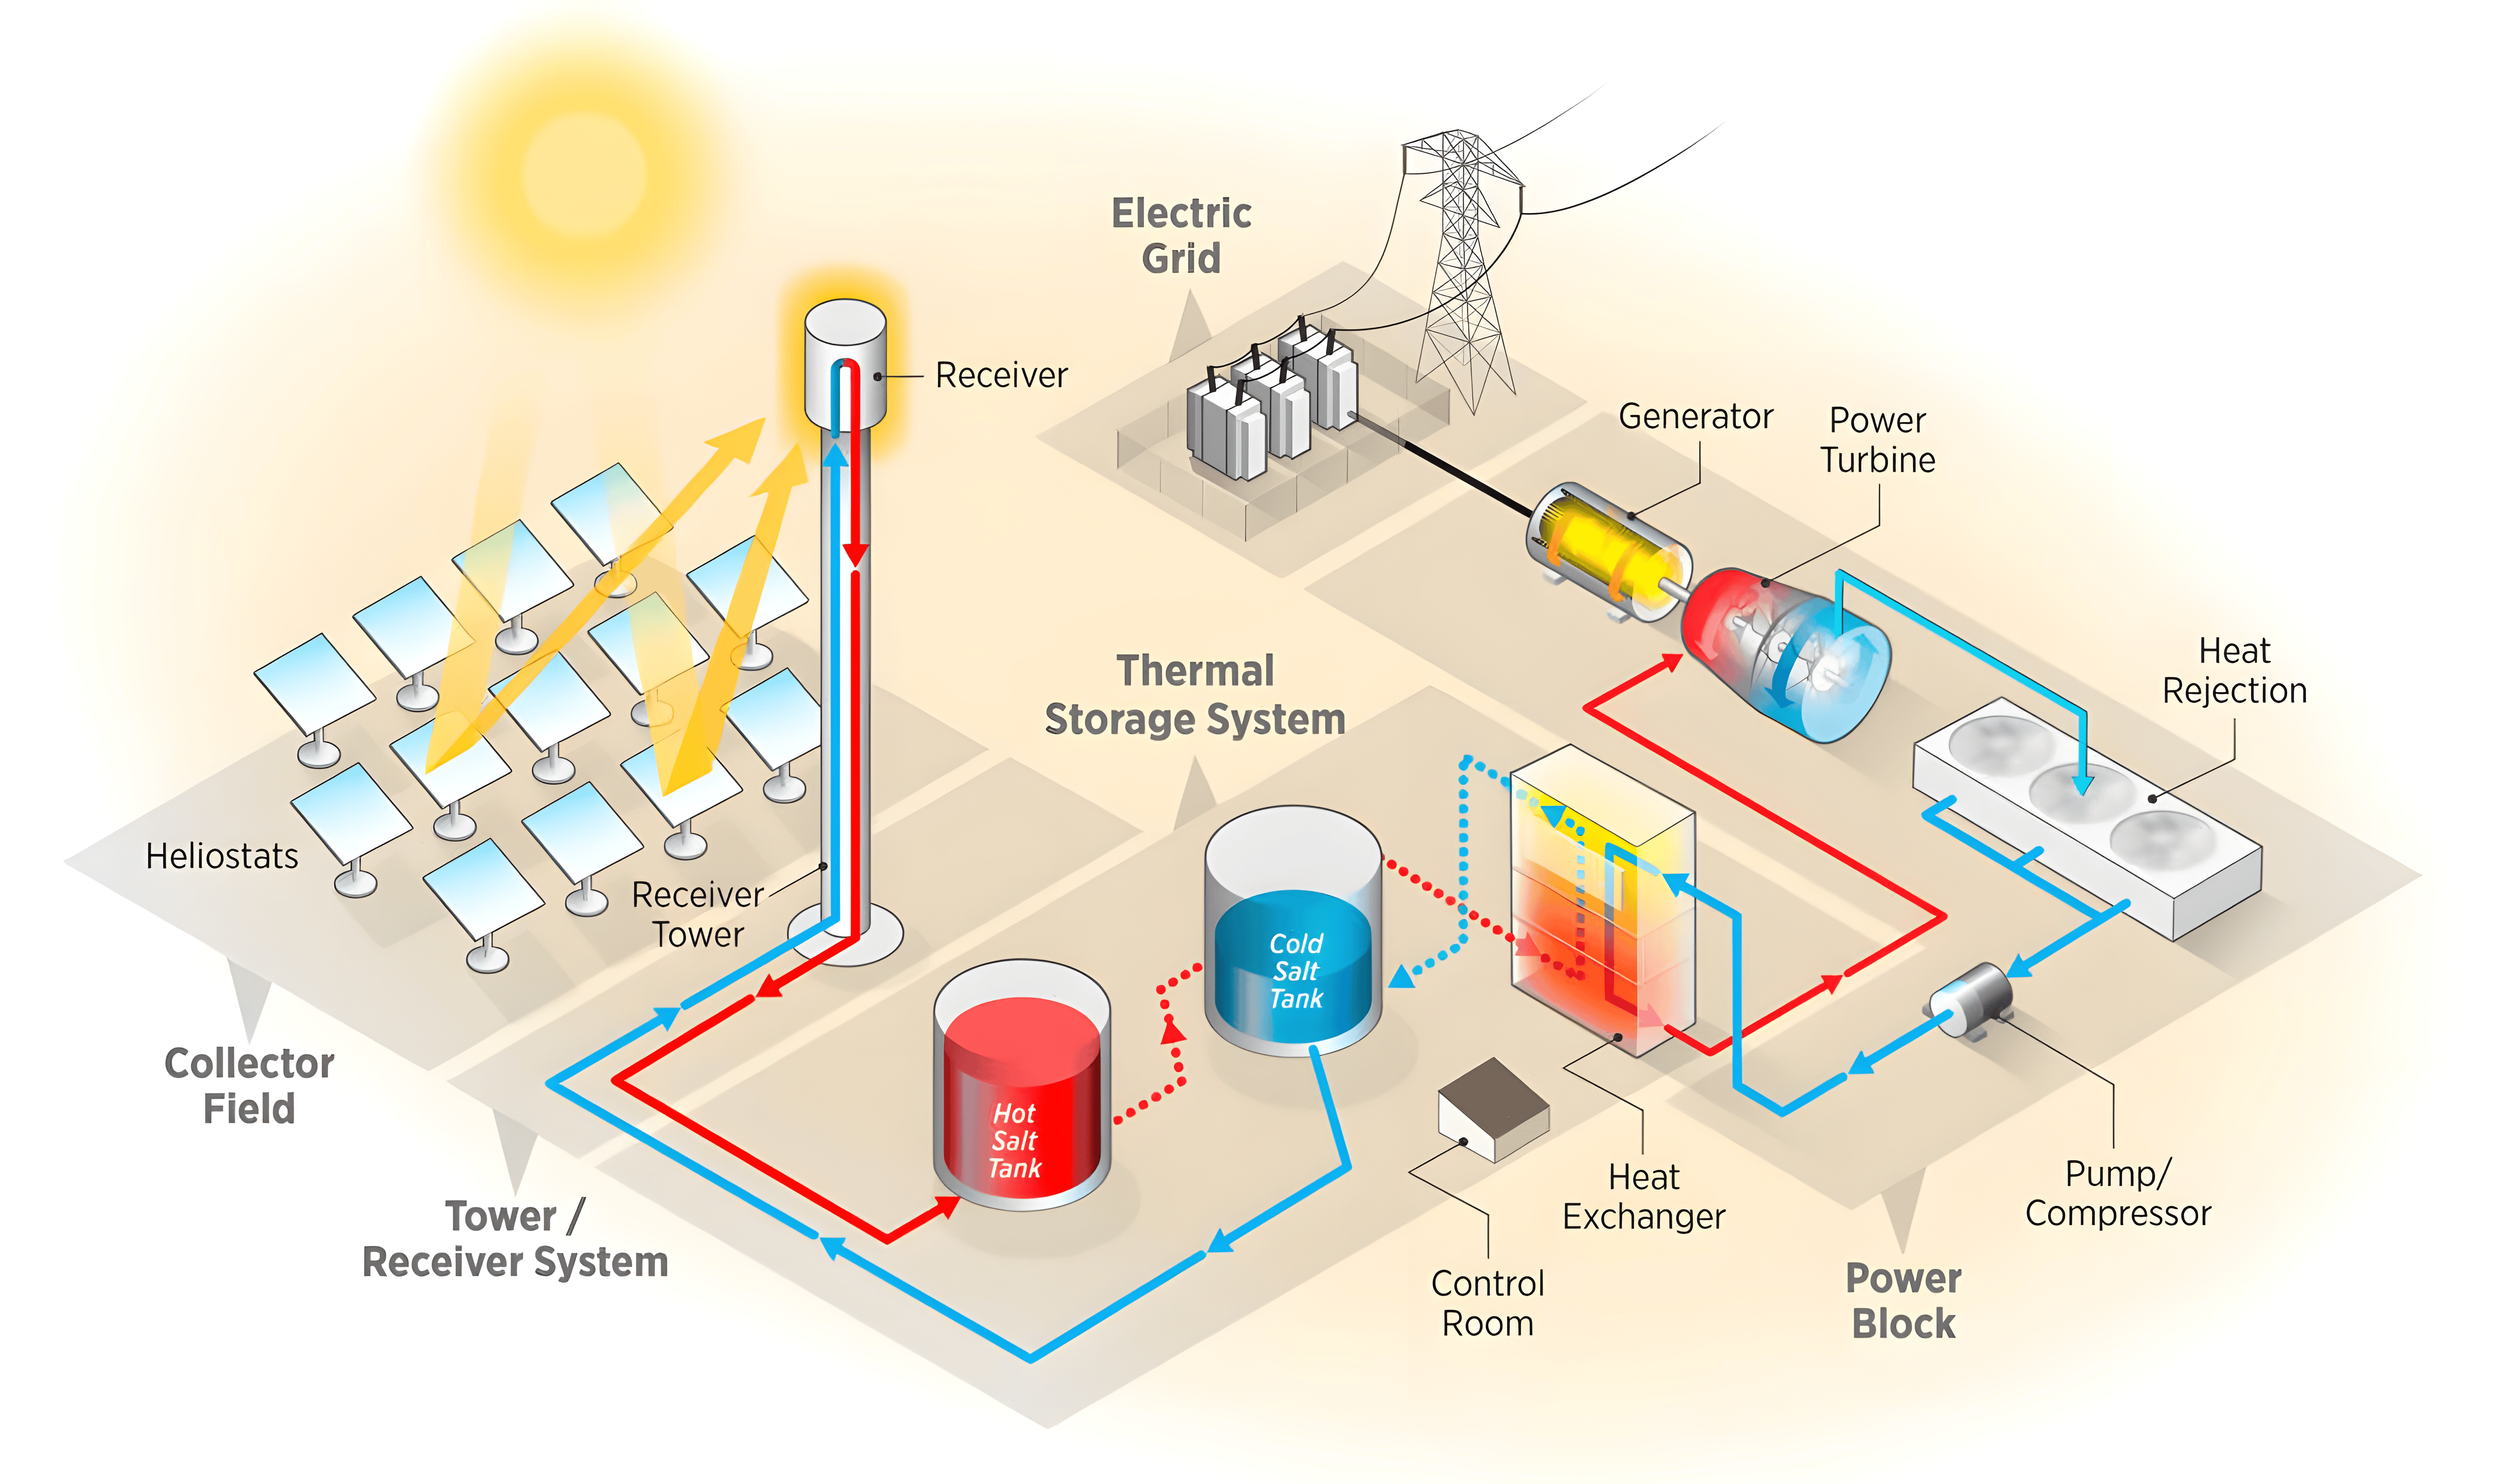
\includegraphics[width=\textwidth]{solar-tower-diagram.png}
    \caption[Solar tower \gls{cspLabel} plant]{Solar tower \gls{cspLabel}
    plant.\\Source: NREL~\cite{mehos_concentrating_2017}}
    \labfig{cc:intro:csp-plant-diagram}
\end{figure}

By coupling \gls{cspLabel} with thermal storage
---\reffig{cc:intro:csp-plant-diagram} - \textit{Thermal Storage System}---
electricity can be generated after sundown or even days later, for example
during adverse weather periods. Because of this ability, \gls{cspLabel} is one
of the few renewable electricity technologies that can generate fully
dispatchable or fully baseload power at very large
scale~\sidecite{pfenninger_potential_2014}. Finally,  the exhaust steam from the
turbine ---\reffig{cc:intro:csp-plant-diagram} - \textit{Power block}--- is
directed to a condenser, where its latent heat of vaporization is transferred to
the available cooling medium. 

\gls{cspLabel} is an engineering-heavy, complex technology, with each project
being different and tailored to both the environment in which it stands and the
requirements of each single
offtaker~\sidecite[*-2]{binz_technologysensitive_2017}. This means, that despite
its relative long history, is still in its formative
phase~\sidecite[*-1]{lilliestam_midterm_2021}\sidenote[][*-15]{In the context of
the industrial life-cycle (ILC)~\cite{bento_measuring_2016}, the formative phase
considers the period in which a technology and its industry and innovation
system are still immature and need to grow and develop}. As \gls{cspLabel} is
not yet competitive with other new generation, and especially not with operating
and depreciated generators, it requires policy support to be economically
viable~\sidecite[]{mirartigues_economics_2019}. This is due to its irregular
historical development.

\subsection{A brief history of \gls{cspLabel}: from the hype to unrealized potential}
\labsec{cc:intro:csp:context}

At one point, \gls{cspLabel} was seen as the leading alternative for large-scale
solar energy. Ambitious visions and bold initiatives—such as the Desertec
project—played a key role in generating immediate excitement around the
technology~\sidecite{schmitt_why_2018}. However, the political consequences of
raising expectations that were ultimately unmet proved significant. In Europe,
this disillusionment contributed to \gls{cspLabel} becoming politically
sidelined for many years~\cite{schmitt_why_2018}. Additionally, around 2010-2012
the cost crossover with \gls{pvLabel} occurred and from there the \gls{pvLabel}
cost advantage only increased~\sidecite{irena_renewable_2025}. Many investments
shifted from \gls{cspLabel} to the more straightforward and profitable
\gls{pvLabel} technology.


The development of \gls{cspLabel} has been marked by alternating periods of
rapid expansion and sharp decline, largely shaped by national policy support. In
the 1980s, California's incentives led to the construction of nine
\gls{cspLabel} plants totaling around 350~MW$_\text{e}$, but the withdrawal of
support caused the bankruptcy of the main developer of solar thermal electric
projects, \textit{Luz}, in 1991, resulting in a 15-year global pause in new
projects. A second growth phase began in 2007 with feed-in tariffs in Spain and
temporary backing in the US, leading to the construction of about 50 plants,
mostly supplied by Spanish and German companies. However, the end of policy
support in both countries around 2013 led to a sharp slowdown, with construction
activity in 2016 at just one-third the 2012 level, and many firms exiting the
sector. \gls{cspLabel} remained commercially active mainly through projects in
Morocco and South Africa, although costs increased and future prospects dimmed.
Momentum returned in 2016 when China introduced a new feed-in tariff aimed at
5~GW$_\text{e}$ of capacity, sparking renewed global interest. Optimism was
further strengthened by major projects launched in Dubai and Morocco in
2018--2019.  The near- to mid-term outlook for \gls{cspLabel} is very uncertain
but there are several positive developments concerning the global value chain
and cost development. The market and policy outlook is bleak with the risk of a
complete loss in many markets for \gls{cspLabel}
~\sidecite{lilliestam_midterm_2021}.


Setting realistic targets may ultimately be more effective than raising
expectations that cannot be met.~\gls{cspLabel} remains a valuable technology
for the energy transition—though likely at a smaller scale than initially
envisioned, and over a longer timeframe. Several studies highlight its potential
role in a zero-carbon or near zero power
system~\sidecite{bonilla_feasibility_2022}. For instance, the \gls{ieaLabel}'s
Net Zero by 2050 report projects that the global \gls{cspLabel} capacity should
reach 73~GW$_\text{e}$ by 2030 and 281~GW$_\text{e}$ by
2040~\sidecite{iea_net_2021}. Likewise, \gls{irenaLabel} envisions several
hundred gigawatts of \gls{cspLabel} by 2050, contributing to grid stability
alongside a projected 8500~GW$_\text{e}$ of solar \gls{pvLabel} and
6000~GW$_\text{e}$ of wind capacity~\sidecite{irena_world_2024}. These
projections suggest that \gls{cspLabel} can play a complementary role to
\gls{pvLabel} and wind by providing dispatchable, on-demand renewable
electricity—further enabling intermittent renewable alternatives. However, even
at these more modest levels, \gls{cspLabel} deployment would need to accelerate
rapidly (see \reffig{cc:intro:csp-lcoe-capacity}~(a)). To meet the
\gls{ieaLabel}'s 2030 target, the global \gls{cspLabel} fleet—standing at just
6~GW$_\text{e}$ in 2021—would need to expand more than tenfold in under a
decade~\sidecite{lilliestam_scaling_2023}.
%[See figure X. La figura esté en el margen y el pie de página describa cuánto
%de cada tecnología está previsto]. [`lilliestam_midterm_2021`](Bibliography/@lilliestam_midterm_2021.md). 
So far this is not happening, \gls{cspLabel} technology remains niche with only
7 plants coming online in the 2020--2023 period~\cite{irena_renewable_2025} and
is unlikely to become a globally important contributor to power system balancing
in the next decade~\cite{lilliestam_scaling_2023}. However, things might be
changing: 4 new plants came online in 2024, the costs of new \gls{cspLabel}
stations have decreased rapidly in the last years, 77~\% from 2010 to 2024,
including a 46~\% reduction from 2023 to 2024 (see
\reffig{cc:intro:csp-lcoe-capacity}~(b)). In terms of \gls{lcoeLabel}, it means
that \gls{cspLabel} has improved from 0.402~$\mathdollar_{2024}$/kWh to below 10
cents (0.092~$\mathdollar_{2024}$/kWh) making it competitive with new fossil
fuel power stations~\sidecite[*-3]{irena_renewable_2025} and the Chinese
\gls{cspLabel} project pipeline includes 37 future and ongoing projects, with a
total capacity of 4.8~GW$_\text{e}$~\sidecite[*-2]{chinasolarthermalalliance_blue_2024}.

\begin{figure*}
    \centering
    \subfloat[\centering Estimated future share of new renewable generation.\\Source: Lilliestam~\etal~\cite{lilliestam_midterm_2021}]{{\includegraphics[width=0.47\linewidth]{renewables-capacity-evolution-schoniger-2022.png}}}%
    \hspace{0.1cm}
    \subfloat[\centering \gls{lcoeLabel} evolution. Source: \gls{irenaLabel}~\cite{irena_renewable_2025}]{{\includegraphics[width=0.47\linewidth]{renewables-lcoe-evolution-irena-2025.png}}}%
    \caption[\gls{lcoeLabel} evolution and capacity predictions]{\gls{lcoeLabel}
    evolution and capacity predictions for different renewable technologies.
    Share is dominated by variable renewable energies and \gls{cspLabel} is the
    fifth largest contributor, serving as a ``gap filler'' for the system
    flexibility of the EU electricity system~\cite{schoniger_need_2022}}
    \labfig{cc:intro:csp-lcoe-capacity}
\end{figure*}

%================================
%================================

\section{Cooling and water use}
\labsec{intro:csp:cooling}

The successful deployment of \gls{cspLabel} plants depends on several key
factors: high annual direct normal irradiance, adequate land availability, and
sufficient water resources. However, while the first two are typically found in
arid regions as shown in \reffig{cc:intro:solar-vs-water-availability}, the
availability of water is often limited. In such locations, the source of raw
water is usually restricted to groundwater or limited surface water bodies such
as rivers, lakes, wells, or artificial reservoirs.


A \gls{cspLabel} plant consumes water for various purposes, with the most
significant demand coming from the cooling of the power
block\sidenote[][*-3]{When wet cooling is used, further explained in the
following}. The power output and efficiency of a thermal power plant are
strongly influenced by the operating temperature and pressure conditions at the
condenser, which are directly linked to the turbine backpressure, and in turn to
the cooling system.

In addition to cooling, water is also required for other plant operations, including~\sidecite[*-4]{rohani_optimization_2021}:

\begin{itemize}
    \item Mirror cleaning (1.3~\% of total water consumption)
    \item Boiler blowdown (1.4~\%)
    \item Miscellaneous uses, auxiliary equipment cooling, and general
    infrastructure and staff needs.
\end{itemize}

In wet-cooled \gls{cspLabel} plants, cooling water accounts for over 95~\% of the
total water consumption, which can be further broken down into evaporation:
77.8~\% and blowdown and drift: 19.1~\%~\cite{rohani_optimization_2021}.


\begin{marginfigure}[-3.5cm]
    \includegraphics[]{cc-intro-water-consumption-comparison.png}
    \caption[Water consumption comparison between thermal power generation technologies]{Water consumption comparison between \gls{cspLabel} and other
    thermal power generation technologies.\\Source: Aseri~\etal~\cite{aseri_condenser_2022}}
    \labfig{cc:intro:water-consumption-comparison}
\end{marginfigure}

Although \gls{cspLabel} plants share a similar power cycle with other thermal
power technologies, their water consumption patterns differ (see
\reffig{cc:intro:water-consumption-comparison}). This is due to their unique
capacity factor, operating schedule, and particularly their strong dependency on
weather conditions, which contrasts with the more stable operation of
fossil-fired plants. Conventional thermal power plants (\eg coal,
gas, or nuclear) are often sited near reliable freshwater sources, such as
rivers or lakes, allowing them to utilize wet cooling without severe resource
constraints. These plants are not tied to solar availability and can prioritize
water access in their location decisions. \gls{cspLabel} plants, however, must
prioritize solar access and land availability and thus have less flexibility
in selecting sites with abundant water.

\begin{figure*}
    \centering

    \subfloat[\centering Solar resource map.\\Source: \href{https://solargis.com/}{Solar resource map\textcopyright2021 Solargis}]{{\includegraphics[width=0.51\linewidth]{cc-intro-ghi-map.png}}}%
    \hspace{0.1cm}
    \subfloat[\centering Water-stress map.\\Source: \href{https://www.wri.org/applications/aqueduct/water-risk-atlas}{Water Risk Atlas © World Resources Institute}~\cite{kuzma_aqueduct_2023}]{{\includegraphics[width=0.44\linewidth]{cc-intro-water-stress-map.png}}}%
    
    \caption[Solar power and water scarcity map]{Greater potential for solar-powered processes takes place in water-scarce regions}
    \labfig{cc:intro:solar-vs-water-availability}
\end{figure*}


%================================
\subsection{Conventional condenser cooling technologies}
\labsec{cc:intro:conventional-cooling}

To date, the conventional systems used to remove excess heat from \gls{cspLabel}
plants are either wet (water-cooled) or dry (air-cooled), each with distinct
characteristics and trade-offs regarding water usage, thermal performance, and
cost.

\reminder{Cooling thermodynamic concepts}{
    \begin{itemize}
        \item The \textit{cooling range} refers to the temperature drop experienced by the cooling water as it circulates through the condenser. The greater the better.
        \item The \textit{approach} of the cooler is the temperature difference between the cooler outlet and the lowest attainable cooling medium temperature, which varies depending on the cooling technology used.
        \item The \fullgls{itdLabel} is the temperature difference between
        the hot fluid entering the cooler and the reference sink (\eg, dry-bulb temperature) at the cooler inlet.
        \item \fullgls{ttdLabel} represents the difference between the outlet
        temperatures of the cooling and the cooled fluids.  
    \end{itemize}
}

\begin{figure*}
    \centering
    
    \subfloat[\centering \fullgls{wctLabel}.\\Source: \href{https://www.evapco.com/products/cooling-towers-factory-assembled/cooling-tower}{EVAPCO}]{{\includegraphics[width=0.3\linewidth]{wet-cooler.png}}}%
    \hspace{0.1cm}
    \subfloat[\centering \fullgls{accLabel}.\\Source: \href{http://www.hzhdss.com/English/case/8970613335.html}{ZMH}]{{\includegraphics[width=0.25\linewidth]{acc.jpg}}}%
    \hspace{0.1cm}
    \subfloat[\centering \fullgls{acheLabel}.\\Source: \href{https://www.alfalaval.com/products/heat-transfer/finned-tube-air-heat-exchangers/finned-tube-air-heat-exchangers/olmi-air-cooler/}{Alfa Laval}]{{\includegraphics[width=0.3\linewidth]{dry-cooler.png}}}%
    
    \caption{Conventional cooling technologies}
    \labfig{cc:intro:conventional-coolers}
\end{figure*}


\subsubsection{Wet cooling}
\labsec{cc:intro:wet-cooling}

Water has traditionally been used as the cooling medium in wet cooling
technology due to its high heat capacity and the possibility of reuse. In power
plants, the steam exiting the turbine is condensed in a surface condenser, where
cooling water circulates through tubes and absorbs the latent heat of the steam.
The warmed cooling water is then returned to the cooling system for heat
rejection, in closed-loop systems, or returned to the body of water in open-loop
(\ie~once-through) systems. In \gls{cspLabel} plants, closed-loop systems are
predominantly used and analyzed in the remaining text.


Wet cooling towers function as heat rejection devices by
bringing warm water from the condenser into direct contact with air. As part of
the water evaporates, it absorbs heat from the remaining liquid, thereby
lowering its temperature. The cooled water is then recirculated back to the
condenser, completing the loop. This process is highly efficient, but it also
leads to water losses from evaporation, drift, and blowdown.

Wet cooling technology requires a substantial amount of water (1.8--4~l/kWh) for
condenser cooling since heat is rejected to the atmosphere through evaporative
cooling~\sidecite{meldrum_life_2013}. While a small share of heat is removed
through sensible air-to-water heat transfer, 80--90~\% of the cooling is achieved
through the latent heat of vaporization~\sidecite{colmenar-santos_water_2014}.

Land availability for cooling systems is often constrained, particularly in
central receiver plants where the solar field surrounds the receiver and
requires unobstructed space for heliostat placement. For this reason, compact
wet cooling designs using forced-draft towers are predominantly employed, such
as the example shown in \reffig{cc:intro:conventional-coolers}~(a).


\begin{kaobox}[title=Wet cooling main characteristics,colback=MediumPurple2!25!white,colbacktitle=MediumPurple2!25!white]
    \begin{itemize}
        \item Water consumption: 1.8--4~l/kWh~\cite{meldrum_life_2013}
        \item Parasitic load: $\approx$0.0165~kW/KWh  or 0.165~\% average annual consumption~\cite{habl_exergoeconomic_}.
        \item Wet cooling consumes similar power along the year but increases its water consumption in the hotter months~\cite{martin_optimal_2013}.
        \item \gls{cspLabel} plants with wet cooling towers consume as much as 1.7x10$^6$~m$^3$ per year of operation~\cite{rohani_optimization_2021}.
        \item Greater available approach, since the lowest attainable temperature is the wet-bulb temperature. 
        \item 55~\% of \gls{cspLabel} plants worldwide make use of wet cooling technology for condenser cooling~\cite{thonig_cspguru_2023,bonilla_csp_2023}
    \end{itemize}
\end{kaobox}

\marginannotation[*-16]{{\gls{cspLabel} plants next to the sea, why not?}}{
	Building \gls{cspLabel} plants near the sea is generally not recommended.  
    Although seawater could serve as an unlimited resource for once-through
    steam condensation, solar radiation is typically lower in coastal areas,
    land prices are higher, and the salty environment accelerates corrosion,
    which can significantly reduces optical efficiency. However, if a suitable
    site is found and feasible mitigation measures are implemented, CSP with
    seawater cooling or \gls{cspLabel}+D(esalination) plants could be a viable
    option~\cite{palenzuela_concentrating_2015} }

\subsubsection{Dry cooling}
\labsec{cc:intro:dry-cooling}

%% Descripción general de sistemas secos %%
In dry cooling, heat is rejected to the surroundings by convection via extended
or finned surfaces or tubes arranged in a row, and each row consists of numerous
cells~\sidecite[*-1]{turchi_parabolic_2010}. In this type of cooling, the warm
water and the ambient air do not have direct contact with each other (as in wet
cooling). Because air is a poor heat transfer medium, the condenser must operate
at a higher temperature and pressure to drive heat out efficiently. This
sensitivity to ambient air temperature leads to elevated turbine back-pressure,
specially during hot weather, reducing thermal efficiency and power output
compared to wet cooling systems. Dry cooling systems can be broadly categorized
as direct or indirect~\sidecite{maulbetsch_comparison_2004}. 

%% Descripción de cada alternativa %%
In direct systems, turbine exhaust steam is delivered straight to an
\gls{accLabel} (see \reffig{cc:intro:conventional-coolers}~(b)), where heat
rejection to the environment occurs in a single step. The steam is condensed
inside finned tubes by ambient air blown across the exterior finned surfaces
arranged in A-frame (forced draft) or delta (induced draft) configuration. This
process relies on latent heat transfer and can employ either mechanical or
natural draft designs. \glspl{accLabel} have been used for nearly 70 years, and
were pioneered in regions as diverse as Western Europe, South Africa and the
Middle East. The largest \gls{accLabel} units in operation is in South Africa
(Medupi) with six fossil-fuel driven 800~MW$_\text{e}$ units on
\glspl{accLabel}~\sidecite{maulbetsch_economic_2012}.

In indirect systems, steam first condenses in a separate condenser, which may be
either a conventional shell-and-tube surface condenser or a barometric
condenser\sidenote{Also known as jet condenser or contact condenser.} 
(direct-contact type), where steam meets a spray of cooling water. The resulting
warm cooling water is then circulated to an \fullgls{acheLabel} (see
\reffig{cc:intro:conventional-coolers}~(c)) for final heat rejection to the
atmosphere. This arrangement introduces an additional heat exchange stage, so
the \gls{acheLabel} handles only sensible heat transfer, requiring greater heat
exchange surface area but being less sensitive to fluctuations in ambient
temperature.

A prominent example of an indirect dry cooling configuration is the Heller
system, named after its inventor Prof.~H.~Heller in Hungary in the
1940's~\sidecite{jaszay_industrial_1958,balogh_hellers_2006}. In the
direct-contact Heller system, steam from the turbine condenses in a barometric
condenser, and the resulting warm cooling water is cooled in an \gls{acheLabel}
before recirculation. Thermal performance is generally comparable to that of an
\gls{accLabel}, but mechanically driven Heller systems tend to have higher
specific electrical consumption because, in addition to fan power, extra pumping
power is required to overcome the jet condenser's added pressure
drop~\sidecite{milman_aircooled_2020}.

If an indirect-contact surface condenser is used instead of a barometric
condenser, the setup is generally less efficient than both \glspl{accLabel} and
the direct-contact condenser Heller configuration because it introduces a
\gls{ttdLabel} (\gls{ttdLabel} $\approx$3--4~$^\circ$C versus
$\approx$0.3~$^\circ$C for barometric condenser), resulting in lower overall
cycle efficiency.

There remains challenges with natural draft dry cooling towers compatibility
with \gls{cspLabel}. For example, in central receiver systems, their significant
size (>~70~m tall, >~60~m~$\varnothing$) would obstruct the heliostat field. A
possible alternative is fan-assisted natural draft systems, which reduce tower
height while retaining some benefits of natural draft
operation~\sidecite{andras_advanced_2005}. Heller systems have been operating
for decades in 17 power plants including the largest indirect dry cooled
combined cycle power plant with 3x777~MW$_\text{e}$ dry towers at
Gebze-Adapazari combined cycle (Turkey)~\cite{andras_advanced_2005}.

%% Costes %%
Unlike wet cooled plants, the dry cooled plants require minimal waterside
infrastructure and other related components. None dedicated to the cooling such
as water supply network, evaporation ponds, storage ponds, biological cooling
water treatment. As a consequence, for the dry-cooled plants, capital and
operation and maintenance costs of these components are
negligible~\cite{maulbetsch_economic_2012}.

However, a recent review on condenser cooling
technologies~\sidecite{aseri_condenser_2022} shows that a dry-cooled
\gls{ptLabel} based plant would deliver 3--10~\% less annual electricity output
and would cost 4~\% to 10~\% more than a wet-cooled plant resulting in 2~\% to
19~\% increase in \gls{lcoeLabel}. It was also observed that due to large
differences in operating temperature of power cycle (560~$^\circ$C for
\gls{stLabel} based plants and 391~$^\circ$C for \gls{ptLabel} based plants),
the reduction in net electricity output for \gls{stLabel} based plants is less
as compared to \gls{ptLabel} based plants (Sau~\etal, 2016). It should be noted
that many of these analysis were made for first generation \gls{cspLabel} with
no thermal storage, which is an outdated technology. The inclusion of thermal
energy storage in the dry or hybrid cooling plant (six hours of storage
capacity) can reduce the overall penalty of \gls{lcoeLabel} considerably: 8.1~\%
to 6.3~\% for dry-cooled as compared to wet-cooled
plants~\cite{aseri_condenser_2022}. According to Maulbetsch et
al.~\sidecite{maulbetsch_comparison_2004}, the \textit{breakeven} water cost at
which wet and dry cooling have the same annual costs (for situations in which
the rest of the base case values and assumptions apply) is between 2 and
3~USD$_{2002}$/kgal.


\begin{kaobox}[title=Dry cooling main characteristics,colback=OliveDrab3!25!white,colbacktitle=OliveDrab3!25!white]
    \begin{itemize}
        \item Capital cost ratio ranges from 4.5 times at a hot, arid site to about 3.5 times at more moderate weather~\cite{maulbetsch_comparison_2004}.
        \item Electrical consumption: 1.5 to 5 times wet cooling, 0.05--0.06~kW$_\text{e}$/kWh
        \item Penalty up to 25~\% during the hottest hour of the year~\cite{maulbetsch_comparison_2004} and 5--6~\% average annual parasitic consumption~\cite{aseri_condenser_2022,martin_optimal_2015,birkinshaw_comparison_2002}.
        \item Limited approach, constrained by the dry-bulb temperature, worsened if an indirect contact surface condenser is used.
        \item 24~\% of commercial \gls{cspLabel} plants make use of this technology~\cite{thonig_cspguru_2023,bonilla_csp_2023}.
        \item Most new plants expected to be built in the next years
        will make use of dry cooling~\cite{chinasolarthermalalliance_blue_2024}. 
    \end{itemize}
    \vspace{1ex}
    \textcolor{darkgray}{\footnotesize\textbf{NOTE:} Comparisons are made relative to wet cooling}
\end{kaobox}


% %================================
\subsection{Non-conventional cooling: Combined / hybrid cooling}
\labsec{cc:intro:combined-cooling}

While energy efficiency has long been a priority, water conservation only began
receiving significant attention in recent years. This is reflected in the large
number of wet-cooled \gls{cspLabel} plants built in the past. Today, some of these plants
face growing scrutiny and competition for water resources, as many regions of
the world experience prolonged periods of water stress. In response, a third
alternative is gaining traction: hybrid or combined cooling technologies, which
integrate the advantages of different cooling methods (wet and dry) into a
single, innovative system. The concept has been explored since the
1970s~\sidecite[*-10]{hu_engineering_1976,zaloudek_study_1976,loscutoff_preliminary_1975,
wiles_description_1978} and regained momentum in the following
decades~\cite{maulbetsch_comparison_2004,maulbetsch_economic_2012}, although
early studies primarily focused on fossil-fuel and nuclear thermal power plants.
Over the past decade, interest sparked in evaluating hybrid cooling solutions
specifically for concentrated solar power systems.


\annotation{Terminology: \textit{Combined} vs \textit{Hybrid} Cooling}{ 
    In the literature, two terms are commonly used to describe cooling systems that
    integrate both wet and dry components: \textit{hybrid} and \textit{combined}.\\
    
    \textbf{Hybrid systems} refer to configurations where the dry and wet
    cooling components are integrated into a single physical unit. An example is
    a cooling tower with two sections ---an upper dry section followed by a wet
    section that can be activated as needed.\\
    
    \textbf{Combined systems} consist of separate, independent dry and
    wet units connected by a hydraulic circuit. Each component is physically
    distinct and operates independently.\\
    
    From a thermodynamic perspective, hybrid and combined systems are
    functionally equivalent. However, hybrid systems tend to be more compact due
    to their integrated design, while combined systems offer greater flexibility
    in component layout and maintenance. Additionally, combined systems are
    often easier to implement in practice, as the individual dry and wet
    components are commercially available off the shelf unlike hybrid units,
    which may require custom design and manufacturing.\\
    
    These differences are not all that important, so the two terms can be used
    interchangeably. \\
    
    \begin{minipage}{0.48\linewidth}
    \centering
    \includegraphics[width=\linewidth]{cc-intro-hybrid-cooler-diagram-no-bg.png}\\
    \small Hybrid cooler
    \end{minipage}
    \hfill
    \begin{minipage}{0.48\linewidth}
    \centering
    \includegraphics[width=\linewidth]{cc-intro-combined-cooler-diagram-no-bg.png}\\
    \small Combined cooler
    \end{minipage}
}

Many heterogeneous hybrid/combined coolers can be found comprising different
components with different arrangements:

\begin{enumerate}
    \item Water-enhanced dry cooling. A dry cooler (usually \gls{accLabel})
    switchable to wet (deluge condenser cell). In the deluged condenser
    configuration, dry-cooling is prioritized until a certain backpressure is
    reached. When this happens water is sprayed wetting the exchanging surfaces,
    which now act equivalently to the packing bed in a wet cooling tower
    \sidecite[*-20]{loscutoff_preliminary_1975,zaloudek_study_1976,wiles_description_1978,golkar_determination_2019,rohani_optimization_2021}.
    The overall heat transfer rates are improved since now the transfer
    mechanism is air to the water film that evaporates, but air-metal contact is
    lost, effectively disabling the dry-cooling mechanism. In this configuration
    is either one or the other. Still, because the nominal cooling capacity of
    such systems is usually achieved by assembling multiple smaller cells, it is
    possible to operate them in parallel. In practice, this means that some
    cells can remain in dry mode (or even be designed exclusively for dry
    operation), while others can be switchable to wet mode when needed. See
    \reffig{cc:intro:hybrid-combined-examples} (a) for an example of such
    system.
    
    \item Dry cooler (usually \gls{accLabel}) + \gls{wctLabel} in parallel
    \sidecite[*-10]{maulbetsch_economic_2012,barigozzi_wet_2011,barigozzi_performance_2014}.
    In this configuration part of the vapor is directed to an \gls{accLabel} while the
    rest goes to a surface condenser cooled by a wet cooling tower. Each cooler
    can be sized independently. A commercial example of such system can be seen
    in \reffig{cc:intro:hybrid-combined-examples} (b).
    
    \item \gls{scLabel} + \gls{acheLabel} + \gls{wctLabel} in series.
    
    \item \gls{scLabel} + (\gls{acheLabel}+\gls{wctLabel}) in
    series-parallel~\sidecite{palenzuela_experimental_2022,
    asvapoositkul_comparative_2014,hu_thermodynamic_2018}. The series-parallel
    configuration is interesting since it offers the greatest degree of
    flexibility, at the cost of adding two heat transfer processes in series, at
    a minimum (\gls{scLabel}$\rightarrow$\gls{acheLabel}), and three if in series
    configuration:
    \gls{scLabel}$\rightarrow$\gls{acheLabel}$\rightarrow$\gls{wctLabel}. Though
    this last one is intended and not so problematic since the wet cooling has a
    higher \gls{itdLabel} (in this case, the difference between outlet
    temperature from dry cooler and wet bulb temperature). Flexibility is
    provided by the almost continuos flexible hydraulic configuration: only
    series, only parallel, any configuration in between or only one of the
    systems. But also in the design, each cooler can be sized
    independently\sidenote{Specially in the combined cooler case, in the hybrid
    alternative it might not be as straightforward}. This allows to optimize the
    system adhoc for each particular deployment by running simulations with the
    expected operation conditions and prioritizing more the wet or the dry
    component. \\An example of such system is shown in
    \reffig{cc:intro:hybrid-combined-examples}~(c).
\end{enumerate}

From a literature review a few conclusions can be drawn:

\begin{itemize}
    \item Air flow rates are very different between dry and wet systems, so any
    design needs to allow independent regulation of each. In the combined
    configuration (separate coolers) this is easily achieved since they have
    independent fans. On the other hand for hybrid systems with a single shared
    fan louvers can be used to regulate the air flow through each
    section~\cite{asvapoositkul_comparative_2014}.
    \item Corrosion might be a problem in the deluged condenser, if so, plastic
    exchange surfaces might have to be used, further decreasing already low heat
    transfer coefficients.
    \item If dry and wet systems share the condenser \ie the hydraulic circuit.
    A direct contact jet-condenser type cannot be used, since the power cycle
    requires high-quality water and large amounts would need to be constantly
    replenished because of the wet cooler evaporation.
    \item If the dry cooler is going to be the main cooling source throughout
    the year, options that combine an \gls{acheLabel} with a surface condenser, are going
    to penalize the dry cooling component compared to alternatives like the \gls{accLabel}
    or Heller system ---both with or without delugement or a parallel only
    configuration.
    \item On the contrary, during operation systems that allow combinations of
    series-parallel configurations provide the greatest potential to adapt the
    cooling system to the changing operation and ambient conditions. The series
    configuration is a water conservative configuration while still being able
    to maintain the required backpressure despite adverse conditions. The
    parallel configuration maximizes cooling capacity but is more water
    intensive.
\end{itemize}

\begin{figure*}
    \centering
    
    \subfloat[\centering Schematic depicting the integration of a deluge
    condenser (wet) cell together with an \gls{accLabel} cell \\ Source:  \href{https://www.minwatercsp.eu/blog-29-full-scale-testing-in-stellenbosch-south-africa/}{ENEXIO
    Management
    GmbH}]{{\includegraphics[width=0.3\linewidth]{minwatercsp_deluge_condenser_ACC-cell.png}}}%
    \hspace{0.1cm}
    \subfloat[\centering A parallel \gls{accLabel}-\gls{wctLabel}. \\ Source:
    Maulbetsch~\etal~\cite{maulbetsch_comparison_2004}]{{\includegraphics[width=0.3\linewidth]{cc-acc-wct-parallel.png}}}%
    \hspace{0.1cm}
    \subfloat[\centering Combined cooling system at \gls{psaLabel}]{{\includegraphics[width=0.35\linewidth]{cc-intro-combined.png}}}%
    
    \caption{Different hybrid/combined coolers configurations}
    \labfig{cc:intro:hybrid-combined-examples}
\end{figure*}

Hybrid/combined cooling technology generally requires larger infrastructure as
it comprises of components of both wet and dry cooling technologies, though much
smaller water side infrastructure~\sidecite{rohani_optimization_2021}. Also, the
potential for water reuse for a hybrid system according to Rohani et
al.~\cite{rohani_optimization_2021} can amount to 23~\% of the total raw water
consumption (mainly due to blowdown). An important part of this water can be
treated and reused without significantly increasing the production costs: up to
14~\% reduction with the same production cost or even slightly reduced.

These systems are a compromise between full-wet and full-dry systems. Due to
their heterogeneity depending on the prioritized objective their costs and
consumptions can be closer to one or the other. Such systems can be sized for a
range of desired water savings. The systems are normally considered for annual
water use targets from 15~\% to 85~\% of that used by a wet cooling system.
Outside that range, they are normally not economically attractive. When even
less water than this is available, water-enhanced dry systems might be the
better option~\cite{maulbetsch_comparison_2004}. For some configurations (when
using indirect dry cooling) they can get more expensive than the standalone
\gls{accLabel} alternative~\cite{maulbetsch_economic_2012}. Finally, the
inclusion of thermal energy storage in the hybrid cooled plant (six hours of
storage capacity) can reduce the overall penalty of \gls{lcoeLabel} from 6.4~\%
to 3.2~\% compared to wet-cooled plants~\sidecite{aseri_condenser_2022}.

\begin{kaobox}[title=Hybrid cooling main characteristics,colback=HotPink3!25!white,colbacktitle=HotPink3!25!white]
    \begin{enumerate}
        \item Capital cost: 2--3.5x~\cite{maulbetsch_economic_2012}
        \item Penalty: 1--3~\%, 2--8~\% in \gls{lcoeLabel}~\cite{aseri_condenser_2022}, 
        \item Just one commercial \gls{cspLabel} plant makes use of this technology~\cite{spx_spx_2012}
    \end{enumerate}

    \vspace{1ex}
    \textcolor{darkgray}{\footnotesize\textbf{NOTE 1}: Due to the novelty
    and heterogeneity of these systems, values can change significantly.}
    \vspace{0.35ex}
    \textcolor{darkgray}{\footnotesize\textbf{NOTE 2}: Comparisons are made
    relative to wet cooling.}
\end{kaobox}


%================================
\subsection{Selection of the cooling technology}[Cooling technology selection]

Selection of condenser cooling technology can affect the financial as well as
technical viability of \gls{cspLabel} plants. These
difference between technologies are dependent on the environment conditions
(local water cost, local temperature, etc.). Except for extreme cases: no water
availability making a dry cooler the only choice or plenty water availability
throughout the year leading to the obvious decision of a wet cooler, this is not
a trivial decision. Dry cooling is increasingly used in \gls{cspLabel} projects,
even though they typically come with higher capital costs and reduced
thermodynamic performance, particularly in hot weather for the dry only
alternative. These systems trade water savings for lower efficiency, making the
choice of cooling technology a critical design decision that balances technical,
economic, and environmental considerations. 

Selecting the cooling technology is not trivial, specially if a hybrid cooler is
chosen. The relative capability of the wet and dry systems is the primary
determinant of the system cost. This, in turn, depends on: the amount of water
available for cooling and the value of plant output during the hottest hours of
the year compared to the average value over the entire year.  As a general rule,
the more water available for cooling, the cheaper and more efficient is the
cooling system. If the amount of water available is between 15\% and 85\% of
that required for an all-wet system, the capital cost of a hybrid system will be
intermediate between the costs of an all-wet and an all-dry
system~\sidecite{maulbetsch_comparison_2004}. Also, environment context and costs
structures are strongly dependent on the particular location and affect
decision-making. Annual simulations of the different cooling alternatives should
be performed using weather data for the particular location, local water
availability throughout the year, and performing a techno-economical analysis in
order to make an informed decision.

So far most systems make use of either wet cooling (55~\% worldwide) or dry
(24~\%)\sidenote{the remaining 21~\% is unknown, but likely to be either of the
conventional technologies}~\sidecite{thonig_cspguru_2023}, but is likely that
some hybrid cooling configuration would be the optimal choice in most situations
where a wet only alternative is used\sidenote{and probably in some dry only ones
too} due to their adaptive nature and flexible operation. Currently, few
commercial plants makes use of hybrid cooling technologies. An example of a
series, integrated, hybrid system providing significant water conservation
exists at the San Juan Generating Station in Farmington, New Mexico. It consists
of a conventional, shell-and-tube steam condenser coupled to a hybrid tower with
an air-cooled dry section on top which discharges into a wet cooling tower
beneath. For \gls{cspLabel}, the only known plant to make use of this technology
is the Crescent Dunes Solar Energy Project, a 110~MW$_\text{e}$ concentrated
solar power station equipped with 1.1~GWh of molten-salt thermal energy storage.
This plant makes use of the described parallel configuration (\gls{accLabel} +
\gls{wctLabel})~\sidecite{spx_spx_2012}. Also, within the \textit{MinWaterCSP}
project, a full scale pilot hybrid plant consisting of an air cooled deluged
condenser was successfully built and tested in Stellenbosch, South
Africa~\sidecite{steinbeis2igmbh_blog_2020}. 
